\documentclass{article}
  %----------------------------------------------------------------------------------------
%	Author:	WangYifu
%	Create Date:	2017-02-14
%	Last Modify:	2018-09-01
%----------------------------------------------------------------------------------------
\usepackage[T1]{fontenc}
\usepackage{fourier}
\usepackage[english]{babel}
\usepackage{amsmath,amsfonts,amsthm}
\usepackage{geometry}
\usepackage{fancyhdr}
\usepackage{listings}
\usepackage{color}
\usepackage[yyyymmdd]{datetime}
\usepackage{graphicx}
\usepackage{float}
\usepackage{titling}
\usepackage{titlesec}
%-------------------------------%
%          Page Style           %
%-------------------------------%
\pagestyle{fancyplain}
\fancyhead{}
\fancyfoot[L]{}
\fancyfoot[C]{}
\fancyfoot[R]{\thepage}
\renewcommand{\headrulewidth}{0pt}
\renewcommand{\footrulewidth}{0pt}
\setlength{\headheight}{13.6pt}
\textwidth=6.5in
\textheight=9.0in
\headsep = 0.1in
\renewcommand{\baselinestretch}{1.2}
\geometry{a4paper,left=2cm,right=2cm,top=2cm,bottom=2cm}

%-------------------------------%
%           Font Size           %
%-------------------------------%
\newcommand{\erhao}{\fontsize{22.1pt}{\baselineskip}\selectfont}
\newcommand{\sanhao}{\fontsize{16.1pt}{\baselineskip}\selectfont}
\newcommand{\sihao}{\fontsize{14.1pt}{\baselineskip}\selectfont}
\newcommand{\xiaosi}{\fontsize{12.1pt}{\baselineskip}\selectfont}
\newcommand{\wuhao}{\fontsize{10.5pt}{\baselineskip}\selectfont}
\newcommand{\setFontSize}[1]{\fontsize{#1}{\baselineskip}\selectfont}
\titleformat{\section}{\sanhao\bfseries}{$\bullet$}{5pt}{}

%-------------------------------%
%             Title             %
%-------------------------------%
\newcommand{\horrule}[1]{\rule{\linewidth}{#1}}
\renewcommand{\dateseparator}{ - }
\def\Assignment{Assignment Title}
\title{
\vspace{-2cm}
\normalfont \normalsize
\textsc{Washington University in St. Louis} \\ [0pt]
\horrule{1pt} \\[0.4cm]
\huge {\bf\Assignment}
}
\author{467261 - Yifu Wang}
\date{\normalsize\today\\\horrule{1pt} \\[0.5cm]}

%-------------------------------%
%           TableList           %
%-------------------------------%
\newcommand{\deflabel}[1]{#1\hfill}
\newenvironment{tlist}[1]{
	\begin{list}{}{
			\settowidth{\labelwidth}{\bf#1}
			\setlength{\leftmargin}{\labelwidth}
			\addtolength{\leftmargin}{\labelsep}
			\renewcommand{\makelabel}{\bf\deflabel}}}{
	\end{list}
}

%-------------------------------%
%             Code              %
%-------------------------------%
\definecolor{gray}{RGB}{191,191,191}
\definecolor{dkgreen}{RGB}{96,139,78}
\definecolor{mauve}{RGB}{206,145,120}

\lstset{ %
	language=C++,                % the language of the code
	% basicstyle=\textheight,           % the size of the fonts that are used for the code
	numbers=left,                   % where to put the line-numbers
	numberstyle=\color{black},  % the style that is used for the line-numbers
	stepnumber=0,                   % the step between two line-numbers. If it's 1, each line 
	% will be numbered
	numbersep=5pt,                  % how far the line-numbers are from the code
	backgroundcolor=\color{gray},      % choose the background color. You must add \usepackage{color}
	showspaces=false,               % show spaces adding particular underscores
	showstringspaces=false,         % underline spaces within strings
	showtabs=false,                 % show tabs within strings adding particular underscores
	frame=false,                   % adds a frame around the code
	rulecolor=\color{gray},        % if not set, the frame-color may be changed on line-breaks within not-black text (e.g. commens (green here))
	tabsize=2,                      % sets default tabsize to 2 spaces
	captionpos=b,                   % sets the caption-position to bottom
	breaklines=true,                % sets automatic line breaking
	breakatwhitespace=false,        % sets if automatic breaks should only happen at whitespace
	keywordstyle=\color{blue},          % keyword style
	commentstyle=\color{dkgreen},       % comment style
	stringstyle=\color{mauve},         % string literal style
}

  \def\Assignment{CES547T - M1}
\begin{document}
\maketitle

\section{Homework}
\begin{tlist}{9}

	\item[2.1(a)]
	Start at $S1$, whenever encounter an $a$, move forward. If there is exactly 2 $a$s in the string, it should stop at $S3$.
	\begin{figure}[H]\centering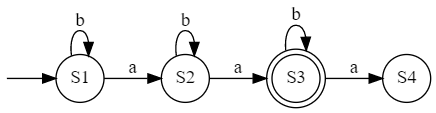
\includegraphics{2_1_a.png}\end{figure}

	\item[2.1(b)]
	Similar to {\bf 2.1 a}, when incounter the 3rd $a$, instead of slipping to $S4$, it stops at $S3$.
	\begin{figure}[H]\centering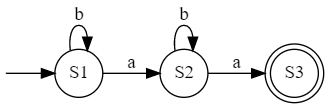
\includegraphics{2_1_b.png}\end{figure}

	\item[4.1(a)]
	$(a+b)^*$
	\begin{tlist}{3}
		\item[1.] $(a+b)^0=\{\Lambda\}\subseteq L(S)$
		\item[2.] Assume $(a+b)^k\subseteq L(S)$. We have
		\begin{align*}
			(a+b)^{k+1} & = (a+b)(a+b)^{k} \\
			            & = (a+b)S         \\
			            & = S
		\end{align*}
		\item[3.] Thus by induction. We have $L(S)=(a+b)^*$.
	\end{tlist}

	\item[4.1(b)]
	$(a+b)^*a$
	\begin{tlist}{3}
		\item[1.] $(a+b)^0a=\{a\}\subseteq L(S)$
		\item[2.] Assume $(a+b)^ka\subseteq L(S)$. We have
		\begin{align*}
			(a+b)^{k+1}a & = (a+b)(a+b)^{k}a     \\
			             & = a(a+b)^ka+b(a+b)^ka \\
			             & = aS+bS               \\
			             & = SS+S                \\
			             & = S+S                 \\
			             & = S
		\end{align*}
		\item[3.] Thus by induction. We have $L(S)=(a+b)^*a$.
	\end{tlist}
\end{tlist}

\section{Quiz}
 (Only simple notes.)
\begin{tlist}{3}

	\item[1.]
	By Cantor's diagonal argument, it's obvious that $[0,1]$ is an uncountable set.

	\item[2.]
	Since every positive rational number can be expressed as
	$$\frac{p}{q} \text{ where } p,q\in\mathbb{N}$$
	Thus $\mathbb{Q}^+=\mathbb{N}\times\mathbb{N}$.

	\item[3.]
	Ridiculous. They are both countable sets. Thus they are both equinumerous to $\mathbb{N}$.

	\item[4.] {\bf(2.1(g))}
	\begin{figure}[H]\centering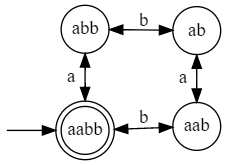
\includegraphics{2_1_g.png}\end{figure}

	\item[5.] {\bf(4.1(c))}
	$b(ab)*$

	\item[6.] {\bf(4.1(h))}
	$\displaystyle\bigcup_{k\text{ is odd}}(a+b)^k$

\end{tlist}
\end{document}